\documentclass[oneside,a4paper,12pt]{article}
\usepackage[english,brazilian]{babel}
\usepackage{multicol}
\usepackage{textcomp}
\usepackage[alf]{abntex2cite}
\usepackage[utf8]{inputenc}
\usepackage[T1]{fontenc}
\usepackage{amsmath,amssymb,exscale}
\usepackage[top=20mm, bottom=20mm, left=20mm, right=20mm]{geometry}%margens cima, baixo, esquerda direita
\usepackage{framed}
\usepackage{booktabs} %Pacote para deixar tabelas mais bonitas.
\usepackage{color} %Pacote de Cores
\usepackage{hyperref} %Pacotes para Hiperlinks
\usepackage{graphicx} %Pacote de imagens
\graphicspath{{./Figuras/}}%Direciona as imagens para uma pasta chamada "Figuras" (uso isso para organizar. Uma vez que todas as imagens vao ficar em uma pasta isolada)    
\definecolor{shadecolor}{rgb}{0.8,0.8,0.8}

%FAZ EDICOES AQUI (somente no conteudo que esta entre entre as ultimas  chaves de cada linha!!!)
\newcommand{\universidade}{Universidade Tecnológica Federal do Paraná}
\newcommand{\centro}{Câmpus Cornélio Procópio}
\newcommand{\departamento}{Departamento Acadêmico de Matemática}
\newcommand{\curso}{Engenharia da Computação}
\newcommand{\professores}{Matheus Pimenta}
\newcommand{\disciplina}{Geometria Analítica e Álgebra Linear - EC31G}
%\newcommand{\tema}{Lista 01}
%\newcommand{\turma}{MA31G}
%\newcommand{\data}{Março de 2019}%{\today}
%\newcommand{\tempodeaula}{30 minutos}
%\newcommand{\prerequisitos}{Matrizes, Transformações Lineares e Bases}
%ATE AQUI !!!	

\begin{document}
	\pagestyle{empty}
	
	\begin{center}
		
\includegraphics[width=\linewidth/8]{logo.jpg}%LOGOTIPO DA INSTITUICAO
	 	\vspace{2pt} 	
		
		\universidade
		\par
		\centro
		\par
		\departamento
		\par
	%	Curso de \curso
		\par
		\vspace{12pt}
		\LARGE \textbf{Lista - Extra}
		
	\end{center}
	
	\vspace{12pt}
	
	\begin{tabular}{ |l|p{12cm}| }
		
		\hline
		\multicolumn{2}{|c|}{\textbf{Dados de Identificação}} \\
		\hline
		Professor:         &    \professores           \\
		\hline
		Disciplina:        &    \disciplina          \\
		\hline
	%	Tema:              &    \tema                \\
	%	\hline
	%	Pré-requisito	:  &    \prerequisitos         \\
	%	\hline
		Aluno:             &                   \\
	%	\hline
	%	Data:              &    \data                \\
	%	\hline
	%	Duração da aula:   &    \tempodeaula         \\
		\hline
		
	\end{tabular}
	\vspace{6pt}
	
	
	\begin{snugshade}
	\end{snugshade}

\begin{enumerate}

	\setcounter{enumi}{33}

	\item Determinar $AA^T$ onde:
	\begin{multicols}{2}
	\begin{enumerate}
		\item $A=\left[
		\begin{array}{ccc}
		1	&	2	&	0	 \\
		3	&	-1	&	4	 \\
		\end{array}
		\right]
		$
		
		{\bf R:}
		$AA^T=\left[
		\begin{array}{cc}
		5	&	1	\\
		1	&	26	\\
		\end{array}
		\right]
		$
	\end{enumerate}
	\end{multicols}

	\item Determinar $A^TA$ onde:
	\begin{multicols}{2}
		\begin{enumerate}
			\item $A=\left[
			\begin{array}{ccc}
			1	&	2	&	0	 \\
			3	&	-1	&	4	 \\
			\end{array}
			\right]
			$
			
			{\bf R:}
			$A^TA=\left[
			\begin{array}{ccc}
			10	&	-1	&	12	\\
			-1	&	5	&	-4	\\
			12	&	-4	&	16
			\end{array}
			\right]
			$
		\end{enumerate}
	\end{multicols}


	\item Prove que $A$ e $B$ são inversas.
	\begin{multicols}{2}
	\begin{enumerate}
		\item $A=\left[
		\begin{array}{ccc}
		1	&	0	&	2	 \\
		2	&	-1	&	3	 \\
		4	&	1	&	8
		\end{array}
		\right]
		$
		
		$B=\left[
		\begin{array}{ccc}
		-11	&	2	&	2	\\
		-4	&	0	&	1	\\
		6	&	-1	&	-1
		\end{array}
		\right]
		$
	\end{enumerate}
	\end{multicols}

	\item Suponha 
	$$A=\left[
	\begin{array}{ccc}
	6	&	-4	&	0	\\
	4	&	-2	&	0	\\
	-1	&	0	&	3
	\end{array}
	\right]
	$$
	
	Determine todas as soluções do tipo $AX = 2X$ e todas as soluções do tipo $AX = 3X$.
	
	\item Para quais valores a tripla ordenada $(y_1,y_2,y_3)$ o sistema $AX=Y$ admite solução, onde:
	$$A=\left[
	\begin{array}{ccc}
	3	&	-1	&	2	\\
	2	&	1	&	1	\\
	1	&	-3	&	0
	\end{array}
	\right]
	$$
	
	\item Para quais valores $(y_1,y_2,y_3,y_4)$ o sistema $AX=Y$ admite solução, onde:
	$$A=\left[
	\begin{array}{cccc}
	3	&	-6	&	2	&	-1	\\
	-2	&	4	&	1	&	3	\\
	0	&	0	&	1	&	1	\\
	1	&	-2	&	1	&	0
	
	\end{array}
	\right]
	$$

	\item Suponha que a placa na Figura \ref{ex01}  represente uma seção transversal de uma barra de metal, com fluxo de calor desprezível na direção perpendicular à placa.
	Sejam $T_1,T_2,\dots,T_6$ as temperaturas em seis vértices interiores do reticulado. A temperatura num vértice é aproximadamente igual à média dos quatro vértices vizinhos  mais próximos. Por exemplo:
	$$T_1 = \frac{(10 + 20 + T_2 + T_4)}{4}$$.
	Estime as temperaturas $T_1,T_2,\dots,T_6$.
	
	\begin{figure}[!h]
		\centering
		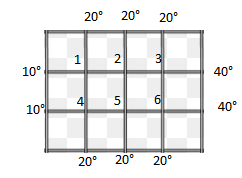
\includegraphics[width=0.4\linewidth]{Figuras/ex01}
		\caption{Malha}
		\label{ex01}
	\end{figure}
	
	{\bf R:} $T_1 = 17,1$, $T_2 = 21,4$, $T_3 = 27,1$, $T_4 = 17,1$, $T_5 = 21,4$ e $T_6 = 27,1$
	
	
\end{enumerate}

	
\end{document}
